\documentclass[11pt]{article}
\usepackage[a4paper,margin=1in]{geometry}
\usepackage{amsmath,amssymb}
\usepackage{graphicx}
\usepackage{booktabs}
\usepackage{xcolor}
\usepackage[hidelinks]{hyperref}
\usepackage{fancyhdr}
\usepackage{titlesec}
\usepackage{enumitem}

\definecolor{mcdblue}{RGB}{20,60,110}
\titleformat{\section}{\large\bfseries\color{mcdblue}}{\thesection}{1em}{}
\titleformat{\subsection}{\normalsize\bfseries\color{mcdblue}}{\thesubsection}{1em}{}
\pagestyle{fancy}
\fancyhf{}
\fancyhead[L]{\small Dual-Band Wilkinson Power Divider -- Wide Frequency Ratio}
\fancyhead[R]{\small MCD Course Project}
\fancyfoot[C]{\thepage}
\renewcommand{\headrulewidth}{0.4pt}

\newcommand{\todobox}[1]{%
  \par\noindent\fbox{\parbox{\dimexpr\linewidth-2\fboxsep-2\fboxrule}{\textbf{\color{red}TODO --- pending EM simulation:} #1}}\par\vspace{4pt}%
}

\title{\color{mcdblue}\textbf{Design of a Dual-Band Wilkinson Power Divider\\ with Wide Frequency Ratio}}
\author{Ghule Yash Mahesh \quad (S20240020288) \\ Himanshu Chandrakant Sinha \quad (S20240020290)}
\date{Microwave Circuit Design Course Project \\ \today}

\begin{document}
\maketitle

\begin{center}
\begin{minipage}{0.85\linewidth}
\small
\textbf{Reference paper:} N.\ Gao, G.\ Wu, Q.\ Tang, ``Design of a Novel Compact
Dual-Band Wilkinson Power Divider With Wide Frequency Ratio,'' \emph{IEEE Microwave
and Wireless Components Letters}, vol.\,24, no.\,2, pp.\,81--83, Feb.\ 2014.
DOI: 10.1109/LMWC.2013.2290226.
\end{minipage}
\end{center}
\vspace{6pt}
\hrule
\vspace{10pt}

\section{Problem Statement}
Design a dual-band equal-split Wilkinson power divider operating at
$f_1 = 500\text{ MHz}$ and $f_2 = 2\text{ GHz}$ (frequency ratio $k=4$), matched and
isolated at both bands simultaneously, using the compact single-line + coupled-line +
lumped-element topology of the reference paper. Target: input/output return loss and
isolation better than 20\,dB at both bands. The design is verified first through
closed-form circuit analysis and MATLAB lossless modeling (Secs.\,2--3), then by a
full-wave EM simulation (Sec.\,4) validated against the lossless model (Sec.\,5).

\section{Mathematical Analysis}
The divider (Fig.\,1 of the reference) consists of a single transmission line
(impedance $Z_1$) from the input port to a junction, splitting into two identical
coupled-line sections (even/odd-mode impedances $Z_e$, $Z_o$) feeding the two output
ports, with an isolation network ($R$, $L$, $C$) connecting the coupled lines'
secondary conductors between the two output ports.

\subsection{Even-mode analysis (input matching)}
With Port 1 excited symmetrically, no current flows in the isolation network, and the
divider reduces to a single branch with the trunk line and the input-port impedance
both doubled (standard bisection for a 2-way equal-split junction):
\begin{align}
Z_{in} &= 2Z_1\,\frac{1+jZ_1\tan\theta}{Z_1+j\tan\theta} \\
Z' &= Z_e\,\frac{Z_{in}+jZ_e\tan\theta}{Z_e+jZ_{in}\tan\theta}
\end{align}
Setting $Z'=1$ (normalized) and separating real/imaginary parts:
\begin{align}
Z_1 Z_e &= 1 \label{eq:ZeZ1}\\
Z_1^2 + 2Z_1^4\tan^2\theta - \tan^2\theta &= 0 \label{eq:quad}
\end{align}

\subsection{Odd-mode analysis (isolation / output matching)}
Driving the two output ports differentially, the symmetry plane becomes a virtual
ground, reducing the circuit to a shorted coupled-line stub (impedance $Z_o$) in
parallel with the bisected isolation network:
\begin{align}
Z_a &= jZ_o\tan\theta \\
Z_b &= \frac{\dfrac{R}{2}\left(\dfrac{1}{j\omega C}+j\dfrac{\omega L}{2}\right)}{\dfrac{R}{2}+\left(\dfrac{1}{j\omega C}+j\dfrac{\omega L}{2}\right)}
\end{align}
Setting $Z'' = \dfrac{Z_a Z_b}{Z_a+Z_b} = 1$ and separating real/imaginary parts:
\begin{align}
R &= 2 \quad\text{(normalized, i.e. } 100\,\Omega \text{ absolute for } Z_0=50\,\Omega)\\
2Z_o\,\omega C\tan\theta + \omega^2 LC &= 2
\end{align}

\subsection{Dual-band design equations}
Requiring input match at both $f_1$ and $f_2=kf_1$ fixes the electrical length of
every line at $f_1$:
\begin{equation}
\theta_{f1} = \frac{\pi}{1+k}, \qquad \theta_{f2} = \frac{k\pi}{1+k}
\end{equation}
Solving the quadratic~\eqref{eq:quad} for $Z_1$ (with $Z_e=1/Z_1$ from
\eqref{eq:ZeZ1}) gives the unique matched line pair. Requiring output match at both
frequencies gives $L$ and $C$ in closed form:
\begin{equation}
L = \frac{2Z_o\tan\theta_{f1}}{\omega_2-\omega_1}, \qquad
C = \frac{\omega_2-\omega_1}{Z_o\,\omega_1\omega_2\tan\theta_{f1}}
\end{equation}
$Z_o$ itself is a free design variable (subject to $Z_o \le Z_e$) that sets the
coupling coefficient of the coupled lines:
\begin{equation}
C(\mathrm{dB}) = -20\log_{10}\!\left(\frac{Z_e+Z_o}{Z_e-Z_o}\right)
\end{equation}
This free parameter is what lets this topology reach band ratios up to 10, unlike
earlier dual-band Wilkinson designs limited to $k<3$. Full derivation with every
intermediate step is in the reference paper, Eqs.\,(1)--(13).

\subsection{Extension: S-parameters vs.\ frequency}
The paper only solves the equations above \emph{at} $f_1$ and $f_2$ (the matched
point). To plot S-parameters across the band (Sec.\,3), the even/odd-mode reflection
coefficients are evaluated at every frequency to get $S_{22},S_{33},S_{23},S_{32}$ via
the standard decomposition:
\begin{equation}
S_{22}=S_{33}=\frac{\Gamma_{even}+\Gamma_{odd}}{2}, \qquad
S_{23}=S_{32}=\frac{\Gamma_{even}-\Gamma_{odd}}{2}
\end{equation}
$S_{11}$ and $S_{21}=S_{31}$ come from the real (undoubled) network: with Port~1
driven and Ports~2/3 terminated at $Z_0$, symmetry still guarantees zero current in
the isolation network, giving a direct closed form for $S_{11}$ and, via an ABCD
cascade of the trunk and branch lines, for $S_{21}$. This was verified against the
paper's own worked numerical example (confirming $S_{11}\approx 0$ and
$|S_{21}|\approx 1/\sqrt{2}$ at $f_1$) before being coded; full derivation is in
\texttt{wilkinson\_model.m}.

\section{MATLAB Lossless Modeling}
Implemented in \texttt{wilkinson\_model.m} (reusable function) and
\texttt{wilkinson\_dualband\_design.m} (design point, self-check, plots).

For $f_1=500$\,MHz, $k=4$, $Z_o$ chosen at $56\,\Omega$ (moderate coupling,
$C(\mathrm{dB})\approx-14.7$\,dB):

\begin{table}[h]
\centering
\begin{tabular}{@{}lr@{}}
\toprule
\textbf{Parameter} & \textbf{Value} \\
\midrule
$Z_1$ & 30.72 $\Omega$ \\
$Z_e$ & 81.38 $\Omega$ \\
$Z_o$ & 56.00 $\Omega$ \\
$L$   & 8.634 nH \\
$C$   & 5.868 pF \\
$R$   & 100.0 $\Omega$ \\
\bottomrule
\end{tabular}
\caption{Solved design parameters, matching the reference paper's own worked example
($Z_1\approx31\,\Omega$, $Z_e\approx81\,\Omega$, $L\approx9$\,nH, $C\approx6$\,pF) to
within rounding.}
\end{table}

\textbf{Self-check} (asserted in code, passes): $S_{11}$, $S_{22}$, $S_{23}$ all below
$-20$\,dB at both 500\,MHz and 2\,GHz.

\begin{figure}[h]
\centering
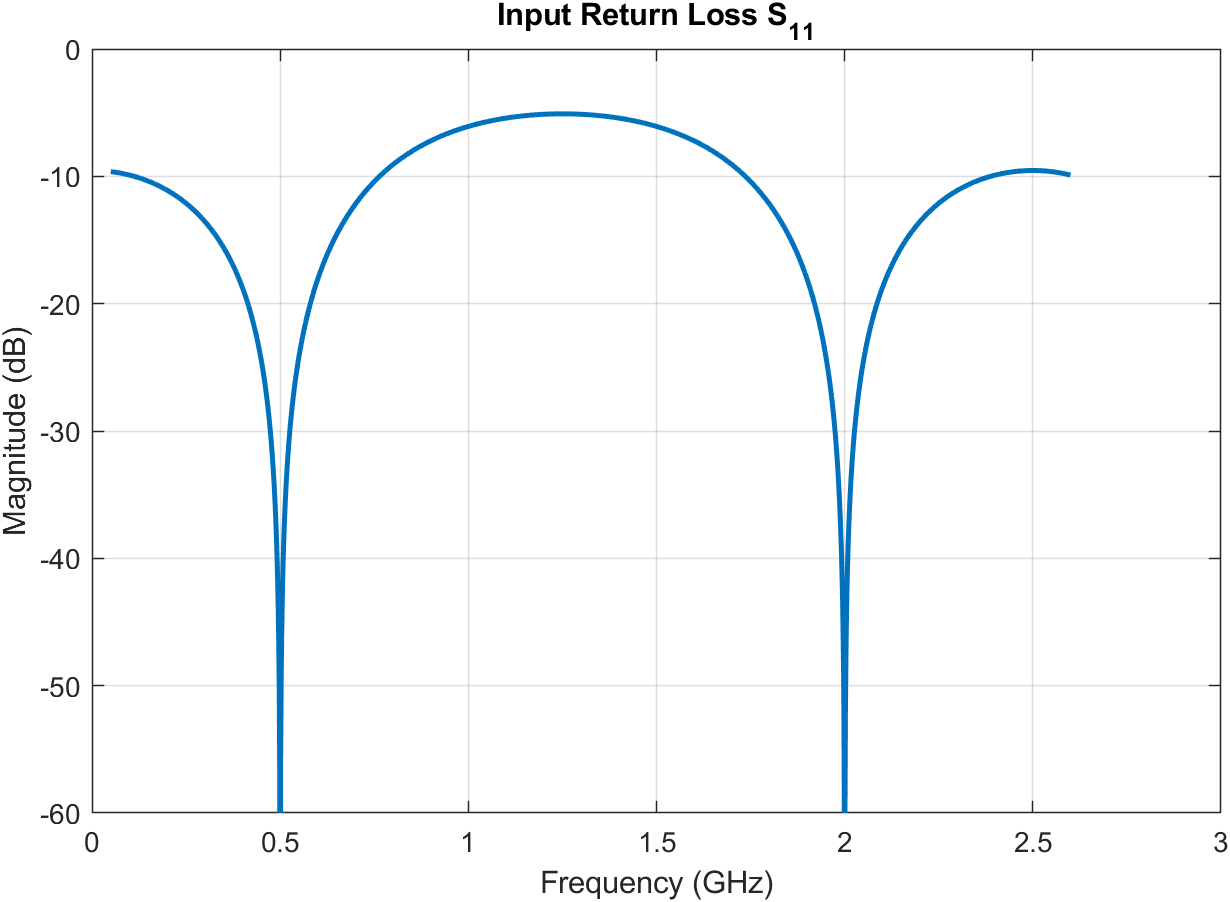
\includegraphics[width=0.48\linewidth]{report_assets/fig_s11.png}
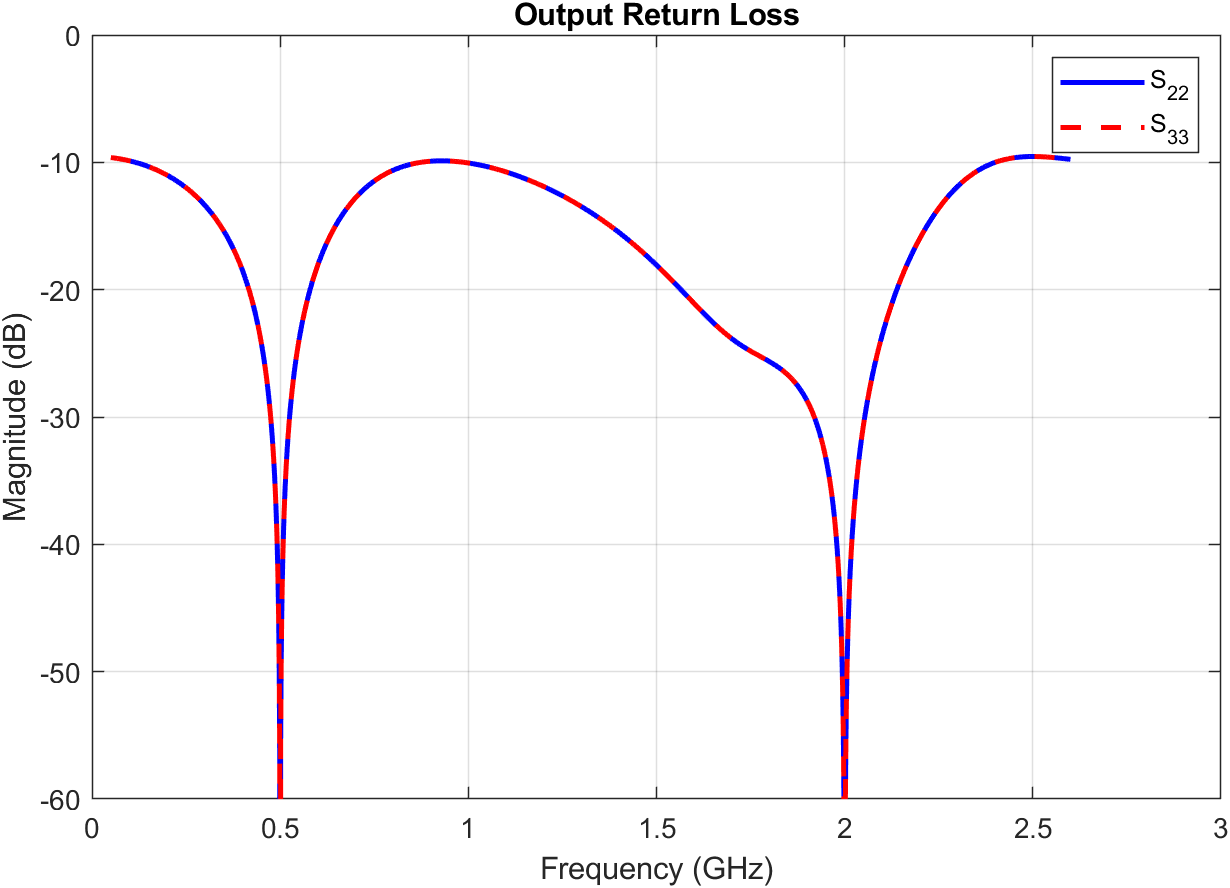
\includegraphics[width=0.48\linewidth]{report_assets/fig_s22.png}\\[4pt]
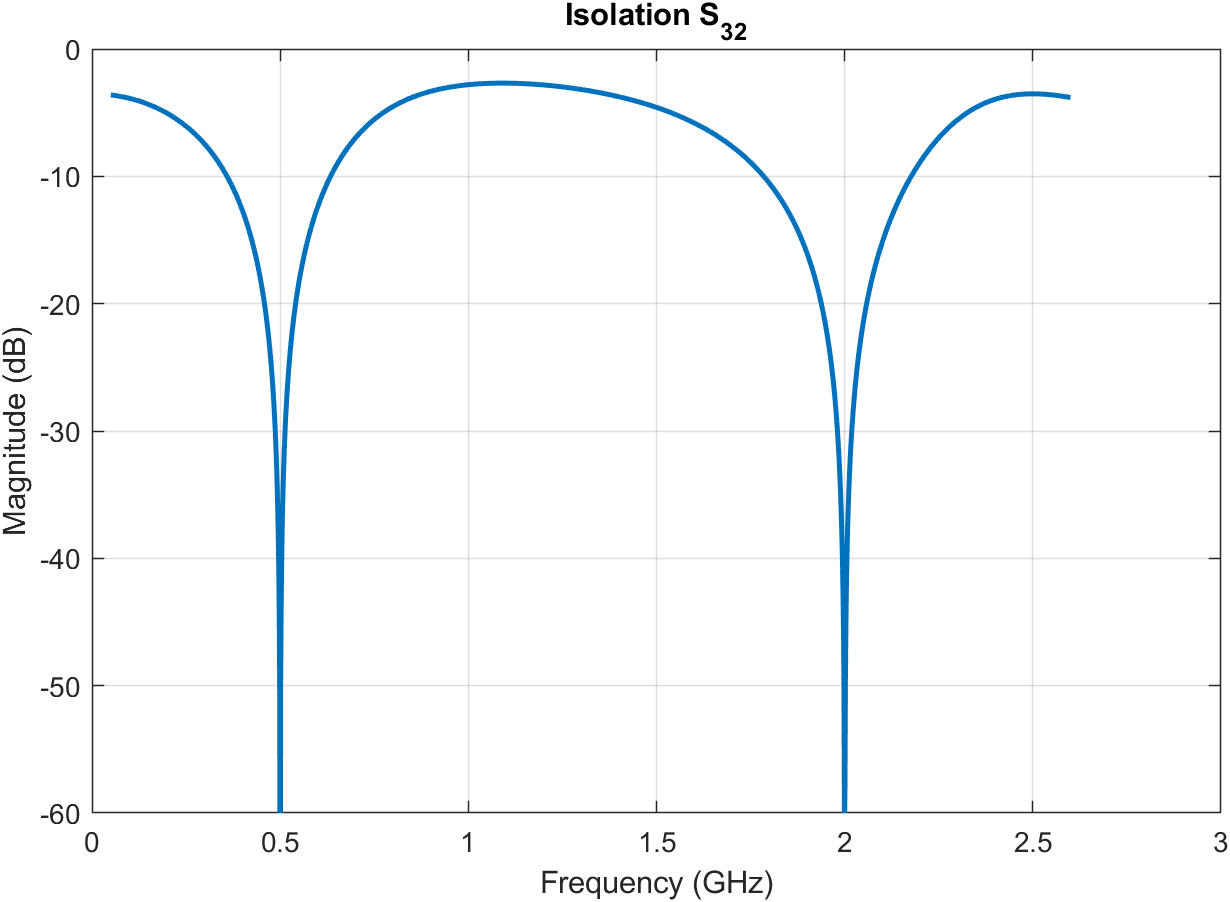
\includegraphics[width=0.48\linewidth]{report_assets/fig_s23.png}
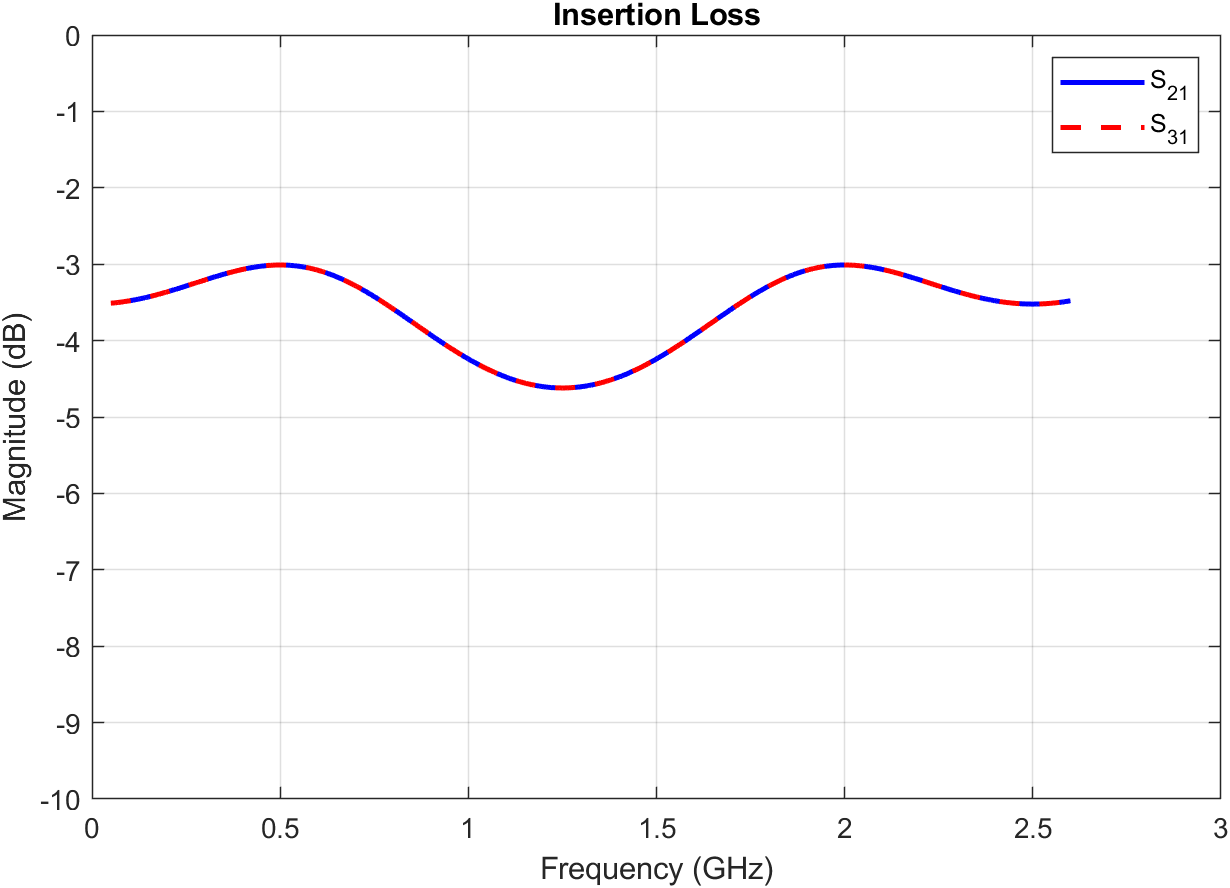
\includegraphics[width=0.48\linewidth]{report_assets/fig_s21.png}
\caption{Lossless MATLAB model: input return loss, output return loss, isolation, and
insertion loss vs.\ frequency. Both passbands (0.5\,GHz and 2\,GHz) show the expected
dual-null return-loss pattern, matching the shape of the reference paper's Fig.\,5.}
\end{figure}

\clearpage
\section{EM Simulation}
\textbf{Substrate:} $\varepsilon_r=2.2$, $h=0.8$\,mm -- matches the reference paper's
fabricated substrate, so the EM layout can also be sanity-checked against the paper's
own measured results as an extra reference point.

\textbf{Starting physical dimensions} (Hammerstad microstrip synthesis,
\texttt{em\_layout.m}, $\theta$ evaluated at $f_1$):

\begin{table}[h]
\centering
\begin{tabular}{@{}lrrrr@{}}
\toprule
\textbf{Line} & $Z_0$ & \textbf{Width} & $\varepsilon_{eff}$ & \textbf{Length (at $f_1$)} \\
\midrule
$Z_1$ (single line)         & 30.72 $\Omega$ & 4.831 mm & 1.947 & 42.998 mm \\
$Z_e$ guess (isolated line) & 81.38 $\Omega$ & 1.094 mm & 1.792 & 44.823 mm \\
$Z_o$ guess (isolated line) & 56.00 $\Omega$ & 2.073 mm & 1.853 & 44.079 mm \\
\bottomrule
\end{tabular}
\end{table}

The $Z_e$/$Z_o$ widths above are \emph{isolated-line approximations only} --
closed-form coupled-microstrip synthesis (Akhtarzad et al.) requires iterating the
width $W$ and gap $S$ simultaneously against both $Z_e$ and $Z_o$, which is more
reliably done with the EM tool's own optimizer than by hand. Starting guess for the
coupled-line pair: $W\approx1.6$\,mm, gap $S\approx h=0.8$\,mm.

\subsection*{HFSS/CST setup steps}
\begin{enumerate}[leftmargin=1.5em]
\item Draw the substrate ($\varepsilon_r=2.2$, $h=0.8$\,mm, copper cladding) and the
three microstrip segments ($Z_1$ trunk, two coupled-line branches) using the
dimensions above as the starting layout.
\item Add the isolation network: two coupling capacitors $C$ to the coupled lines'
secondary conductors, inductor $L$ between them to a center node, resistor $R$ across
the two ends (lumped components, per the $L,C,R$ values in Sec.\,3).
\item Define 3 wave ports (or lumped ports) at Port~1, Port~2, Port~3, reference
impedance $50\,\Omega$.
\item Set up a frequency sweep covering $\sim$0.1--2.6\,GHz (same range as the MATLAB
sweep).
\item Run an optimization (HFSS Optimetrics / CST Optimizer) on the coupled line's $W$
and gap $S$, targeting $Z_e=81.38\,\Omega$ and $Z_o=56.00\,\Omega$ -- or directly
targeting the $S_{11}$/$S_{22}$ minima at 500\,MHz and 2\,GHz.
\item Export the 3-port S-parameters as Touchstone (\texttt{.s3p}) over the full
swept band.
\end{enumerate}

\todobox{Insert EM-simulated S-parameter plots and final tuned dimensions here once
the HFSS/CST run is complete.}

\section{Validation}
\texttt{validate\_em.m} overlays the MATLAB lossless-model curves against the
EM-simulated Touchstone file (\texttt{em\_results.s3p}) automatically once it is
exported from HFSS/CST -- run it after Sec.\,4 to produce the comparison plots.

\todobox{Insert overlay plots ($S_{11},S_{21},S_{22},S_{23}$ -- MATLAB vs.\ EM) and
discuss where/why they diverge. Expected sources of difference: conductor and
dielectric loss (the MATLAB model is lossless), radiation/parasitic coupling at the
T-junction and coupled-line discontinuities, and non-ideal lumped $R/L/C$ parasitics --
none of which are in the closed-form model.}

\section{Conclusion}
\todobox{Summarize after Sec.\,5 -- did the design meet the $>$20\,dB return
loss/isolation target at both bands in simulation? How closely did EM match the
lossless model? What would you change for a second iteration?}

\section*{References}
\begin{enumerate}[leftmargin=1.5em]
\item N.\ Gao, G.\ Wu, Q.\ Tang, ``Design of a Novel Compact Dual-Band Wilkinson Power
Divider With Wide Frequency Ratio,'' \emph{IEEE MWCL}, vol.\,24, no.\,2, pp.\,81--83,
2014.
\item \textit{(Add any textbook/EM-tool documentation references used for the layout
synthesis.)}
\end{enumerate}

\section*{Contribution Statement}
\textit{Fill in honestly based on who actually did what -- required by the course
instructions.}
\begin{table}[h]
\centering
\begin{tabular}{@{}lp{7cm}@{}}
\toprule
\textbf{Task} & \textbf{Contributor(s)} \\
\midrule
Paper selection and problem statement & \\[4pt]
Mathematical derivation (Sec.\,2) & \\[4pt]
MATLAB modeling and plots (Sec.\,3) & \\[4pt]
EM layout and simulation (Sec.\,4) & \\[4pt]
Validation and writeup (Secs.\,5--6) & \\[4pt]
\bottomrule
\end{tabular}
\end{table}

\end{document}
